\documentclass[intlimits, 9pt, unicode]{beamer}

\mode<presentation>
\usepackage[T2A]{fontenc}
%\usepackage[cp1251]{inputenc}
\usepackage[utf8]{inputenc}
\usepackage[russian]{babel}
\usepackage{graphicx}
\usepackage{amssymb}
\usepackage{amsthm}

\usefonttheme[onlymath]{serif}
\newcommand{\textblue}[1]{\textcolor{blue}{#1}}

\usepackage{beamerthemesplit}

\usetheme{Warsaw}
%\setbeamertemplate{page number in head/foot}[totalframenumber]

\setbeamercovered{transparent}
\beamertemplatenavigationsymbolsempty

\setbeamertemplate{footline}{%
\hfill \insertframenumber{}/\inserttotalframenumber\ \ \ \ }

%\setbeamerfont{footline}{series=\bfseries}
%\setbeamertemplate{footline}[frame number]

\title{Обнаружение разладки во временных рядах показов мобильной рекламы}
\author{К.В. Мерзляков, группа 622}
\institute{Санкт-Петербургский Государственный Университет \\
     Кафедра статистического моделирования
}
\date{
    18.05.2019
}

\AtBeginSection[]{
  \begin{frame}
  \vfill
  \centering
  \begin{beamercolorbox}[sep=8pt,center,shadow=true,rounded=true]{title}
    \usebeamerfont{title}\insertsectionhead\par%
  \end{beamercolorbox}
  \vfill
  \end{frame}
}


\begin{document}

\begin{frame}
    \titlepage
\end{frame}

\begin{frame}
    \frametitle{Содержание}



    \begin{itemize}
    	\item Общие замечания
    \vspace{0.5cm}
	 \item Построение модели данных
    \vspace{0.5cm}
        \item Методы обнаружения разладки
    \vspace{0.5cm}
        \item Оценка качества
    \vspace{0.5cm}
        \item Моделирование данных
    \vspace{0.5cm}
        \item Применение моделей к смоделированным данным
    \end{itemize}


\end{frame}



\section{Общие замечания}


%\begin{frame}
%    \frametitle{Изменения в данных}
%
%       \begin{columns}
%    \begin{column}{0.25\textwidth}
%    \centering
%     Запрос
%     \begin{figure}
%	\includegraphics[height=1cm]{images/scheme_request}
%     \end{figure}
%     \end{column}
%    \begin{column}{0.001\textwidth}
%    \centering
%	>
%     \end{column}
%    \begin{column}{0.25\textwidth}
%    \centering
%    Показ
%     \begin{figure}
%	\includegraphics[height=1cm]{images/scheme_impression}
%     \end{figure}
%    \end{column}
%    \begin{column}{0.001\textwidth}
%    \centering
%    >
%    \end{column}
%    \begin{column}{0.25\textwidth}
%    \centering
%    Клик
%     \begin{figure}
%	\includegraphics[height=1cm]{images/scheme_click}
%     \end{figure}
%    \end{column}
%    \begin{column}{0.001\textwidth}
%    \centering
%    >
%    \end{column}
%    \begin{column}{0.25\textwidth}
%    \centering
%     Конверсия
%     \begin{figure}
%	\includegraphics[height=1cm]{images/scheme_conversion}
%     \end{figure}
%     \end{column}
%     \end{columns}
%
%             \vspace{1.2cm}
%
%       {\begin{columns}
%        \begin{column}{5cm}
%        Изменения на стороне пользователя
%         \begin{itemize}
%    		\item Популярность приложения
%		\item Конкуренция
%		\item Маркетинговая активность приложения
%		\item ...
%   	 \end{itemize}
%        \end{column}
%
%        \begin{column}{5cm}
%        Изменения на стороне рекламной сети
%         \begin{itemize}
%    		\item Релиз новых функций
%		\item Партнерство с новыми рекламодателями
%		\item Новые способы таргетинга
%		\item ...
%   	 \end{itemize}
%	 \end{column}
%    \end{columns}}
%
% \end{frame}


%\begin{frame}
%    \frametitle{Временные ряды}
%	
%    {\begin{columns}
%        \begin{column}{5.5cm}
% Временной ряд это ряд, состоящий из числовых значений упорядоченных по времени. Как правило, с равными промежутками времени между значениями (минута, час, день, неделя и т.д.)
% 
%
%\vspace{0.3cm}
%\begin{table}[h!]
%\centering
% \begin{tabular}{||c c||}
% \hline
% Time & Data \\ [0.5ex]
% \hline\hline
% 18-Май-2019 19:00 & 435 098 \\
% \hline
% 18-Май-2019 20:00 & 431 248  \\
% \hline
% 18-Май-2019 21:00 & 420 329  \\
% \hline
% ... & ... \\ [1ex]
% \hline
%\end{tabular}
%\end{table}
%
%	
%\vspace{0.3cm} Формальное обозначение:
% $ X = (x_1, x_2, ... , x_{N-1} , x_N)  $
%
%        \end{column}
%
%\hspace{-0.5cm}
%        \begin{column}{5cm}
%Обычно, временной ряд может быть представлен в виде суммы его компонент $X = T + S + E$
%        \begin{figure}
%        \centering
%	\textbf{Временной ряд. Пример разложения ряда на компоненты}
%        \includegraphics[height=5cm]{images/impressions_stl_6}
%	\end{figure}
%	
%        \end{column}
%    \end{columns}}
%\end{frame}

\begin{frame}
    \frametitle{Разладка во временных рядах}

    \begin{itemize}
    	\item Разладкой во временных рядах называют момент времени, в который произошло существенное изменение в структуре временного ряда
	\item Методы обнаружения разладки --- это группа методов, с помощью которых можно находить такие точки разладки
	\item Разладка может быть двух типов
		\begin{itemize}
			\item Локальная --- аномалия или выброс
			\item Глобальная --- изменение структуры ряда
		\end{itemize}
    \end{itemize}

    {\begin{columns}
        \begin{column}{5cm}
        \begin{figure}
        \centering
	\textbf{Локальная разладка}
        \includegraphics[height=3.5cm]{images/local_cp}
	\end{figure}
        \end{column}

        \begin{column}{5cm}
	\begin{figure}
    	\centering
	\textbf{Глобальная разладка}
        \includegraphics[height=3.5cm]{images/global_cp}
	\end{figure}
        \end{column}
    \end{columns}}

\end{frame}


\begin{frame}
    \frametitle{Мотивация}
    \begin{itemize}
    	\item{Исторические данные}
	    \begin{itemize}
	      \item{Прогнозирование}
	      \item{Извлечение тренда}
	      \item{Поиск проблем в исторических данных}
	    \end{itemize}
    	\item Текущие данные
	    \begin{itemize}
	      \item{Реакция на изменения своевременно}
	    \end{itemize}
    \end{itemize}


   \begin{columns}
        \begin{column}{5cm}
	\begin{figure}
		\textbf{Извлечение тренда без анализа разладок}
		\includegraphics[height=3.5cm]{images/trend_fallacy}
	\end{figure}
        \end{column}

        \begin{column}{5cm}
	\begin{figure}
		\textbf{Извлечение тренда с анализом разладок}
		\includegraphics[height=3.5cm]{images/trend_succeed}
	\end{figure}
        \end{column}
    \end{columns}

%Что можно сделать после обнаружения разладки:
%    \begin{itemize}
%    	\item Убрать/изменить выбросы
%	\item Разбить временной ряд на отрезки и анализировать каждый отдельно
%    \end{itemize}

\end{frame}


\begin{frame}
    \frametitle{Виды разладок}

\begin{columns}
 \begin{column}{0.5\textwidth}

  \begin{columns}
      \begin{column}{0.3\textwidth}
      \centering
      Изменение в тренде
      \end{column}
      \begin{column}{0.5\textwidth}
      \begin{figure}
		\includegraphics[scale=0.08]{images/examples_trend}
	\end{figure}
	\end{column}
     \end{columns}

  \begin{columns}
      \begin{column}{0.3\textwidth}
      \centering
      Изменение в среднем
      \end{column}
      \begin{column}{0.5\textwidth}
      \begin{figure}
		\includegraphics[scale=0.08]{images/examples_mean}
	\end{figure}
	\end{column}
     \end{columns}

  \begin{columns}
      \begin{column}{0.3\textwidth}
      \centering
      Изменение в амплитуде колебаний
      \end{column}
      \begin{column}{0.5\textwidth}
      \begin{figure}
		\includegraphics[scale=0.08]{images/examples_variance}
	\end{figure}
	\end{column}
     \end{columns}

	\end{column}

 \begin{column}{0.5\textwidth}

  \begin{columns}
      \begin{column}{0.3\textwidth}
      \centering
      Локальное изменение
      \end{column}
      \begin{column}{0.5\textwidth}
      \begin{figure}
		\includegraphics[scale=0.08]{images/examples_outlier}
	\end{figure}
	\end{column}
     \end{columns}

  \begin{columns}
      \begin{column}{0.3\textwidth}
      \centering
      Изменение в периодике
      \end{column}
      \begin{column}{0.5\textwidth}
      \begin{figure}
		\includegraphics[scale=0.08]{images/examples_periodic}
	\end{figure}
	\end{column}
     \end{columns}

	\end{column}
	
     \end{columns}

\end{frame}

\begin{frame}
    \frametitle{Структура исследования}

    \begin{itemize}
    	\item Смоделировать данные, близкие к реальным
    \vspace{0.5cm}
	 \item Применить к смоделированным данным набор методов
    \vspace{0.5cm}
        \item Оценить и сравнить качество примененных методов
    \end{itemize}


\end{frame}




\section{Построение модели данных}

\begin{frame}
\frametitle{Данные мобильной рекламы}

   \begin{columns}
    \begin{column}{0.25\textwidth}
    \centering
     Запрос
     \begin{figure}
	\includegraphics[height=1cm]{images/scheme_request}
     \end{figure}
     \end{column}
    \begin{column}{0.001\textwidth}
    \centering
	>
     \end{column}
    \begin{column}{0.25\textwidth}
    \centering
    Показ
     \begin{figure}
	\includegraphics[height=1cm]{images/scheme_impression}
     \end{figure}
    \end{column}
    \begin{column}{0.001\textwidth}
    \centering
    >
    \end{column}
    \begin{column}{0.25\textwidth}
    \centering
    Клик
     \begin{figure}
	\includegraphics[height=1cm]{images/scheme_click}
     \end{figure}
    \end{column}
    \begin{column}{0.001\textwidth}
    \centering
    >
    \end{column}
    \begin{column}{0.25\textwidth}
    \centering
     Конверсия
     \begin{figure}
	\includegraphics[height=1cm]{images/scheme_conversion}
     \end{figure}
     \end{column}
     \end{columns}

   \begin{columns}
    \begin{column}{0.5\textwidth}
	\begin{figure}
	\textbf{Типичный будний день}\par\medskip
	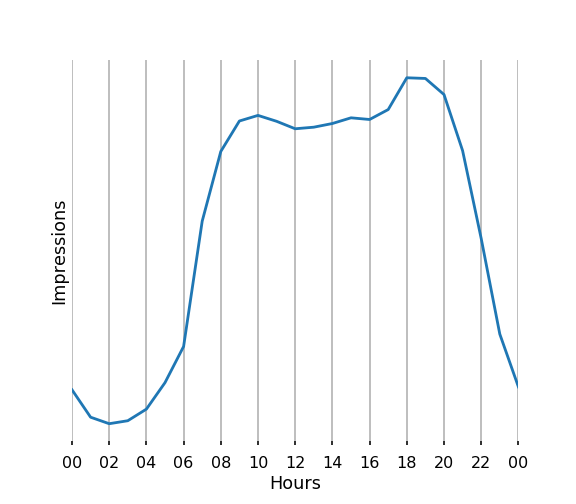
\includegraphics[height=4.5cm]{images/examples_day}
	\end{figure}
     \end{column}
    \begin{column}{0.5\textwidth}
	\begin{figure}
	\textbf{Типичный выходной день}\par\medskip
	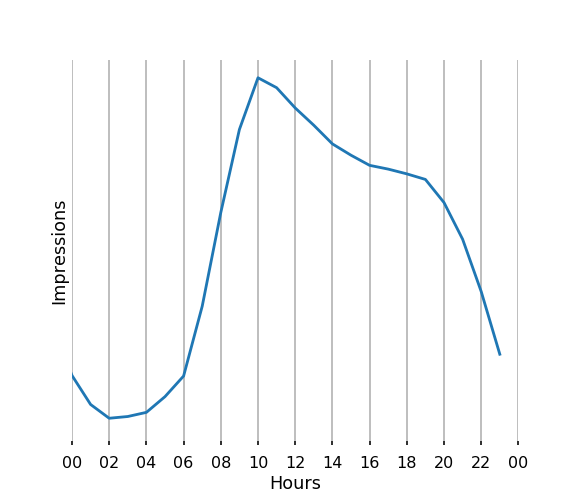
\includegraphics[height=4.5cm]{images/examples_weekend}
	\end{figure}
     \end{column}
     \end{columns}

\end{frame}

\begin{frame}
\frametitle{Примеры разладки в реальных данных}
\begin{figure}
\textbf{Изменение в среднем}\par\medskip
\includegraphics[scale=0.30]{images/1_examples_mean}
\end{figure}
\end{frame}

\begin{frame}
    \frametitle{Построение модели ряда}

    \begin{itemize}
    	\item Обозначим временной ряд $Y = (y_1, \dots, y_n)$
    \vspace{0.5cm}
	 \item Наблюдаемые значения можно представить в виде $Y = T + S + E$, где  $ T = (t_1, \dots, t_n) $ компонента-тренд, $ S = (s_1, \dots, s_n) $ периодическая компонента, $ E = (\epsilon_1, \dots, \epsilon_n) $ остатки или шум
    \vspace{0.5cm}
        \item Для каждой из этих компонент требуется построить модель
    \end{itemize}

\end{frame}


\begin{frame}
    \frametitle{Построение модели ряда}

Модель можно задать следующим образом:
\begin{equation*}
t_i = c, \quad i = 1, \dots, n, 
\end{equation*}

\begin{equation*}
s_i = \sum_{j=1}^{J}{A_j \cos \left( \frac{2\pi}{a_j} i + \phi_j \right)}, \quad i = 1, \dots, n,
\end{equation*}

\begin{equation*}
\epsilon_i \sim N(0, \sigma^2), \quad i = 1, \dots, n, 
\end{equation*}
где $i$ индекс элемента ряда; $j$ индекс косинуса в периодической компоненте; J --- количество косинусов в периодической компоненте; $c$ --- константа; $A_j$ --- амплитуда $j$-го косинуса; $a_j$ --- период $j$-го косинуса; $\phi_j$ --- фаза $j$-го косинуса.

\end{frame}


\begin{frame}
    \frametitle{Модель разладки. Изменение в среднем}

Модель разладки можно задать следующим образом:
\begin{itemize}
	\item Разладка только в одной точке ряда;
	\item Разладка заключается в сдвиге.
\end{itemize}
$\tau$ --- точка (индекс) разладки, тогда тренд с разладкой $ \tilde{T} = (\tilde{t_1}, \dots, \tilde{t_n}) $, где
\begin{equation*}
\tilde{t_i} =
	\begin{cases}
		t_i, & i < \tau, \\
		t_i + \delta^{(mean)}, & i \geqslant \tau,
	\end{cases}
\end{equation*}

$ \delta^{(mean)} $  --- значение разладки. Чтобы разладка была заметна, введем ещё минимальное допустимое значение разладки $\delta_{min}^{(mean)}$, так что:

\begin{equation*}
\delta^{(mean)} = \max(\delta^{(mean)*}, \delta_{min}^{(mean)} ),
\end{equation*}
\begin{equation*}
\delta^{(mean)*} \sim N(\mu^{\mathrm{(cp\_mean)}}, \sigma^{2\mathrm{(cp\_mean)}}).
\end{equation*}



%\delta^{(mean)} = \begin{cases}
%    		\delta^{(mean)*}, & \textrm{с вероятностью } \rho, \\
%  		0, & \textrm{с вероятностью } 1 - \rho.
%	\end{cases} 
%\end{equation*}

\end{frame}

\begin{frame}
    \frametitle{Модель разладки. Локальная}

Отличие от предыдущего типа разладки в том, что в локальной разладки разладка влияет только на одну точку ряда.
\begin{equation*}
\tilde{t_i} =
	\begin{cases}
		t_i, & i \neq \tau, \\
		t_i + \delta^{(local)}, & i = \tau,
	\end{cases}
\end{equation*}

\begin{equation*}
\delta^{(local)} = \max(\delta^{(local)*}, \delta_{min}^{(local)} ),
\end{equation*}
\begin{equation*}
\delta^{(local)*} \sim N(\mu^{\mathrm{(cp\_local)}}, \sigma^{2\mathrm{(cp\_local)}}).
\end{equation*}

Остальное остается идентичным предыдущему варианту.

\end{frame}


%\begin{frame}
%    \frametitle{Модель разладки. Изменение в тренде}
%
%Модель разладки можно задать следующим образом:
%\begin{itemize}
%	\item Разладка только в одной точке ряда;
%	\item Разладка только в тренде и заключается в изменении коэффициента тренда;
%	\item Разладка может произойти не всегда, а с некоторой вероятностью $\rho$.
%\end{itemize}
%$\tau$ --- точка (индекс) разладки, тогда тренд с разладкой $ \tilde{T} = (\tilde{t_1}, \dots, \tilde{t_n}) $, где
%\begin{equation*}
%\tilde{t_i} =
%	\begin{cases}
%		t_i, & i < \tau, \\
%		t_{\tau - 1} + \delta^{(trend)}(i - \tau + 1), & i \geqslant \tau,
%	\end{cases}
%\end{equation*}
%
%$ \delta^{(trend)} $  --- значение разладки. Чтобы разладка была заметна, введем ещё минимальное допустимое значение разладки $\delta_{min}^{(trend)}$
%
%
%Таким образом, независимо от типа разладки, моделируемый ряд с разладкой будет иметь следующий вид:
%%\begin{equation*} Y = e^{\tilde{T} + S + E}.  \end{equation*}
%\begin{equation*}
%%\tilde{Y} = e^{\tilde{T} + S + E}. 
%\tilde{Y} = \tilde{T} + S + E. 
%\end{equation*}
%
%
%\end{frame}

\section{Методы обнаружения разладки}


\begin{frame}
    \frametitle{Общая канва}

\begin{itemize}
	\item У временного ряда есть некоторая структура (сигнал)
	\item Сигнал может быть описан моделью
	\item Идея подхода: около точки разладки модель плохо описывает
временной ряд
	\item Используя меру ошибки мы можем измерять насколько хорошо описывает выбранная модель реальные данные
	\item Как только ошибка (отклонение
модели от реальных данных) превышает заданный порог, метод сигнализирует о разладке
\end{itemize}


Можно выделить два типа методов в данном подходе:
\begin{itemize}
	\item Методы на основе прогнозирования
	\item Методы на основе аппроксимации
\end{itemize}

\end{frame}


\begin{frame}
    \frametitle{Моделируемый ряд и функции рядов в методе разладки}

Исходная модель ряда одна:

\begin{equation*}
Y = T + S + E = c + \sum_{j=1}^{J}{A_j \cos \left( \frac{2\pi}{a_j} i + \phi_j \right)} + \epsilon_i, \quad i = 1, \dots, n, 
\end{equation*}



Моделей сигнала для обнаружения разладки может быть много. Мы будем использовать следующие:
\begin{itemize}
	\item $ f(x | b) = b $
	\item $f(x | P, p, \chi, b) = P\cos(\frac{2\pi}{p}x + \chi) + b$
	\item $f(x | \{P_j, p_j, \chi_j\}, b) = \sum_{j=1}^JP_j\cos(\frac{2\pi}{p_j}x + \chi_j) + b$
\end{itemize}

\end{frame}



\begin{frame}
    \frametitle{Аппроксимация}

Пусть $l$ --- ширина окна. При этом  $ 1 < l < n $, $l$ чётное. С помощью ширины окна из исходного ряда образуется последовательность отрезков $W = \{ w_j \}_{j=1}^k$, где $k = n - l + 1$ --- количество таких отрезков; а $ w_j = (y_j, \dots, y_{j+l-1}) $ --- $j$-ый отрезок. Каждый отрезок  $w_j$  в свою очередь делится на два отрезка одинаковой длины: $ W^{\mathrm{(left)}} = \{w_j^{\mathrm{(left)}} \}  =  \{(y_j, \dots, y_{j+\frac{l}{2}-1}) \}$ и $W^{\mathrm{(right)}} = \{w_j^{\mathrm{(right)}} \} = \{(y_{j+\frac{l}{2}}, \dots, y_{j+l-1}) \}$.

Таким образом, для каждого ряда $W$ можно сформировать тройки рядов: 

\begin{equation*}
W^{\mathrm{(all)}} = \{w_j^{\mathrm{(all)}} \}_{j=1}^k =  \{(w_j; w_j^{\mathrm{(left)}}; w_j^{\mathrm{(right)}}) \}_{j=1}^k. 
\end{equation*}

\end{frame}

\begin{frame}
    \frametitle{Аппроксимация}

Пусть есть функция ошибки $e(\cdot)$, такая что:
\begin{equation*}
e(X) = \min_{\theta}{\sum_{p=1}^m(x_p - f(x_p | \theta))^2 },
\end{equation*}
где $X = (x_1, \dots, x_m)$ ---  вещественный временной ряд длины $m$, а $f(x | \theta)$ --- модель сигнала этого временного ряда с параметрами $\theta$.

%Функция $f(x|\theta)$ может быть константной ($\theta = (b)$):
%\begin{equation*}
%f(x | b) = b,
%\end{equation*}
%либо другой подходящей под наш ряд функцией, например:
%\begin{equation*}
%f(x | P, p, \chi, b) = P\cos(\frac{2\pi}{p}x + \chi) + b. 
%\end{equation*}

\end{frame}

\begin{frame}
    \frametitle{Аппроксимация}

Мера ошибки позволяет нам рассчитать, насколько хорошо аппроксимируется отрезок ряда с помощью выбранной модели. Однако, необходимо еще ввести функцию разладки:
\begin{equation*}
f_j = F(w_j^{\mathrm{(all)}} ) = \frac{e(w_j) - e(w_j^{\mathrm{(left)}}) - e(w_j^{\mathrm{(right)}})}{h}, 
\end{equation*}
где $h$ --- значение нормировки, $j = 1, \dots, k$.

Синхронизация: $f_1$ соответствует $y_l$, а $f_k $ соответсвует $y_n$. Введем синхронизированную функцию разладки :

\begin{equation*}
q_i =
	\begin{cases}
		f_{i-l+1}, & i \geq l, \\
		0, & i < l.
	\end{cases}
\end{equation*}

%Нормирующую константу можно рассчитывать как среднее от ненормированных значений функции разладки на первых отрезках ряда (предполагая, что в начале ряда не происходило разладок):
%\begin{equation*} 
%h = \frac{\sum_{j=1}^{v}e(w_j) - e(w_j^{\mathrm{(left)}}) - e(w_j^{\mathrm{(right)}})}{v} + 1, 
%\end{equation*}
%где $v$ --- сколько отрезков в начале ряда мы используем для расчета $h$.

\end{frame}

\begin{frame}
    \frametitle{Аппроксимация}

\begin{itemize}
	\item Итого, взяв ряд $Y$, мы «скользим» по нему окном ширины $l$
	\item Рассчитываем значения функции разладки $F()$ для каждого из получаемых отрезков $W^{\mathrm{(all)}}$
	\item Функция разладки начинает расти в окрестности точки разладки $\tau$,
	\item Следовательно можно задать порог $\gamma$, такой что при превышении функции разладки этого порога в какой-то точке $\hat{\tau}$, разладка будет обнаружена
\end{itemize}

 \begin{columns}
    \begin{column}{0.3\textwidth}
	\begin{figure}
	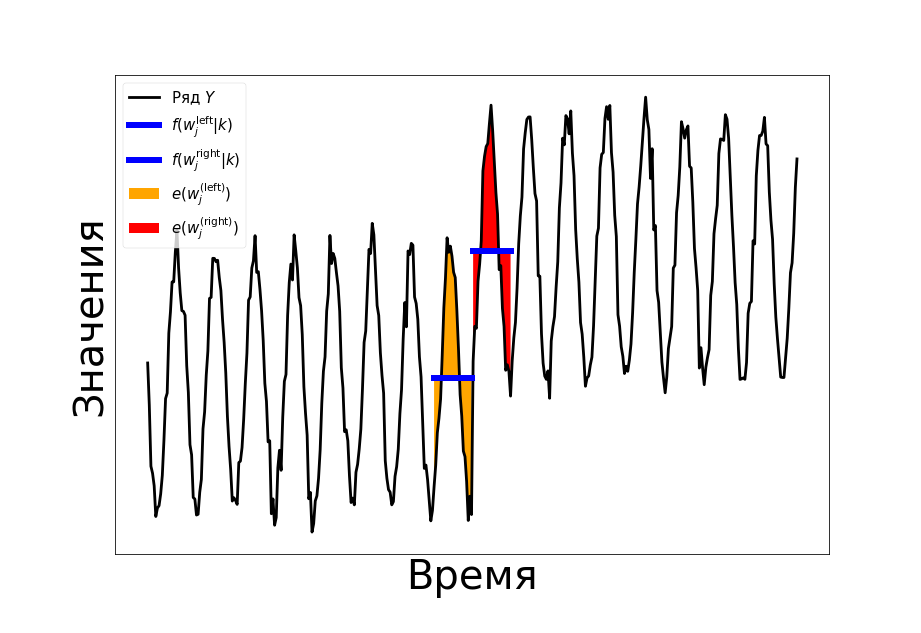
\includegraphics[height=3cm]{images/approaches_second_2_ru}
	\end{figure}
     \end{column}
    \begin{column}{0.3\textwidth}
	\begin{figure}
	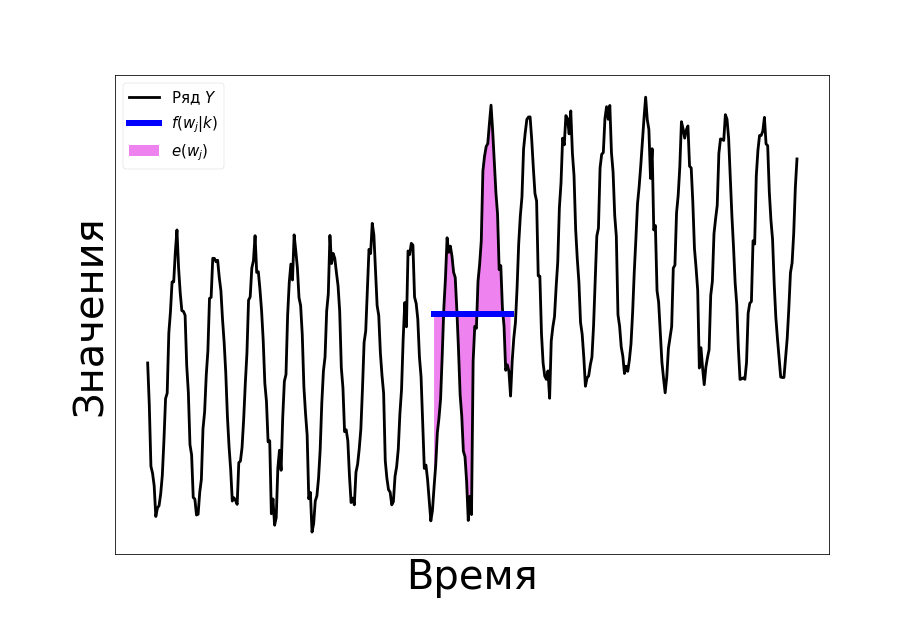
\includegraphics[height=3cm]{images/approaches_second_3_ru}
	\end{figure}
    \end{column}
    \begin{column}{0.3\textwidth}
	\begin{figure}
	\includegraphics[height=3cm]{images/approaches_second_4_ru}
	\end{figure}
    \end{column}
     \end{columns}

\end{frame}


\begin{frame}
    \frametitle{Прогнозирование}

\begin{itemize}
	\item Строим прогноз на несколько точек ряда вперед и считаем отклонение фактических значений от прогнозных
	\item В случае, если отклонение выше заданного порога, метод обнаруживает разладку
	\item Формально, оставаясь в тех же обозначениях, есть та же ширина окна $l$ 
	\item Есть последовательность отрезков $W = \{ w_j \}_{j=1}^k$
	\item  Каждый отрезок  $w_j$ делится в этом методе на два ряда не обязательно одинаковой длины
	\item  Введем индекс $g$, который будет указывать в какой точке ряда $w_j$ он будет разделен на два
	\item  формируется набор из пар рядов:  $ W^{\mathrm{(left)}} = \{w_j^{\mathrm{(left)}} \}  =  (y_j, \dots, y_{j+g})$ и $W^{\mathrm{(right)}} = \{w_j^{\mathrm{(right)}} \} = (y_{j+g}, \dots, y_{j+l})$
\end{itemize}

\end{frame}

\begin{frame}
    \frametitle{Прогнозирование}


Ключевое отличие от методов аппроксимации: вместо расчета меры ошибки на том же ряду на котором подбирались параметры модели, мы оцениваем параметры $\theta$ модели $f(x|\theta)$ на ряде $ w_j^{\mathrm{(left)}} $, делаем прогноз на $ l - g $ точек и рассчитываем функцию ошибки $ e(\cdot) $ на ряде $ w_j^{\mathrm{(right)}} $. Функция разладки принимает следующий вид:
	\begin{equation*}
	 f_j = F(w_j^{\mathrm{(right)}}) = \frac{e(w_j^{\mathrm{(right)}})}{h}.
	 \end{equation*}

\begin{columns}
    \begin{column}{0.5\textwidth}
	\begin{figure}
	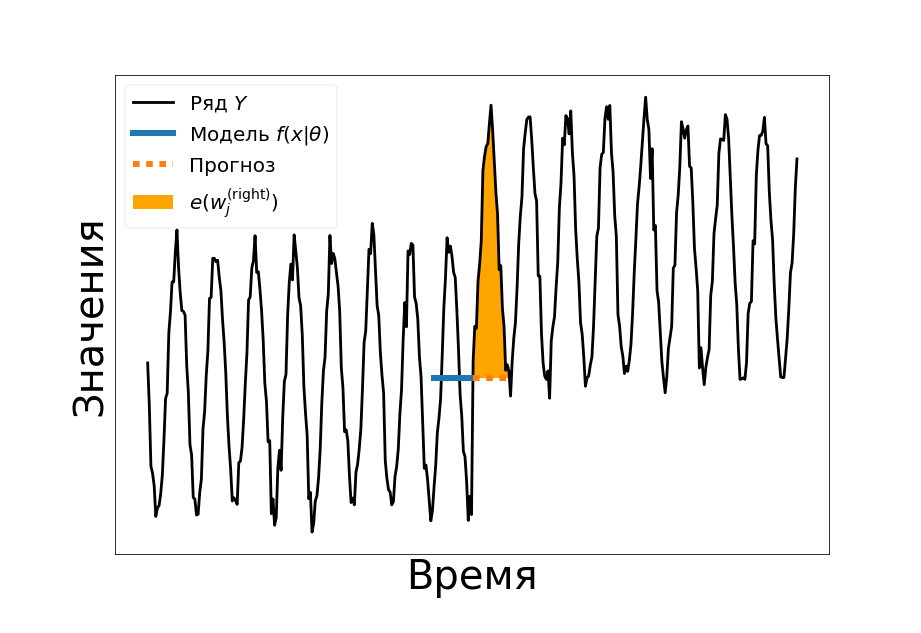
\includegraphics[height=3.8cm]{images/approaches_first_4_ru}
	\end{figure}
     \end{column}
    \begin{column}{0.5\textwidth}
	\begin{figure}
	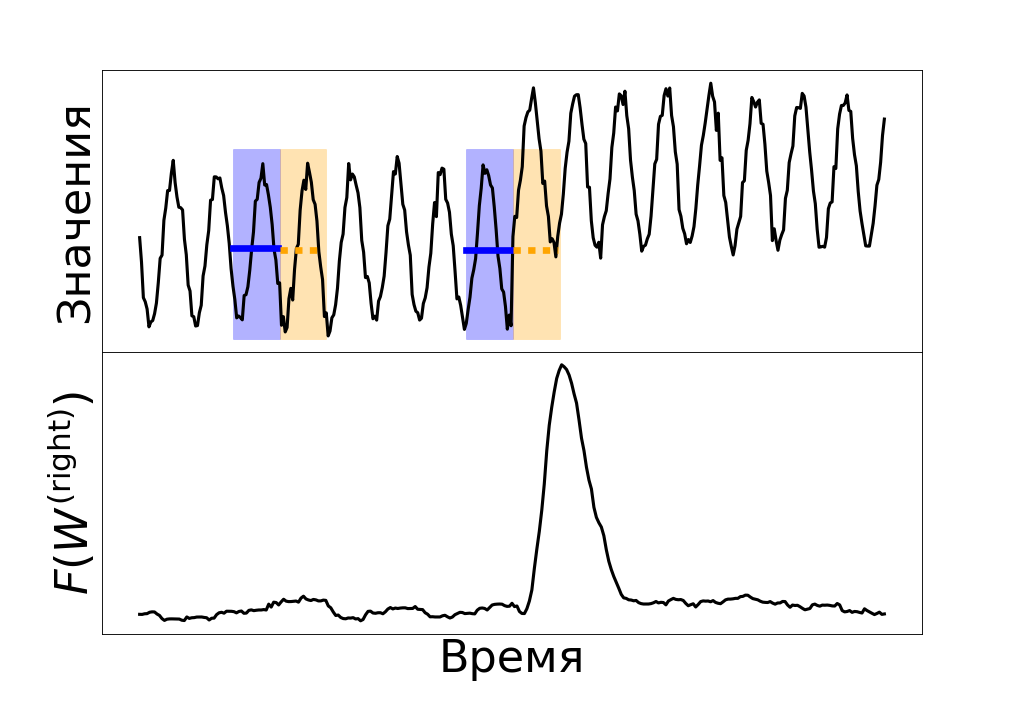
\includegraphics[height=3.8cm]{images/approaches_first_6_ru}
	\end{figure}
     \end{column}
     \end{columns}

\end{frame}

\section{Оценка качества}

\begin{frame}
    \frametitle{Допущения}

В рамках данной работы мы разрабатываем систему своевременного оповещения о разладках во временных рядах.

\begin{itemize}
	\item Нам важны две характеристики: точность и скорость обнаружения разладки
	\item Нам точно известны ряды с разладками и без
	\item Можем строить матрицы ошибок классификации и считать метрики качества
	\item Мы фиксируем точку разладки $\tau$ и приемлемую задержку $d$
\end{itemize}

\end{frame}


\begin{frame}
    \frametitle{Матрица ошибок классификации}

Таким образом, у нас имеется приемлемая задержка, в рамках которой мы хотим обнаружить разладку. При этом, за пределами приемлемой задержки нас не интересует что происходит с рядом.
Исходя из этого возможны четыре варианта:
\begin{itemize}
	\item Разладка произошла и метод обнаружил точку разладки в диапазоне $(\tau, \cdots, \tau+d)$. Такая ситуация попадает под категорию True positive.
	\item Разладка произошла и метод не обнаружил точку разладки в диапазоне $(\tau, \cdots, \tau+d)$. Это случай False negative.
	\item Метод обнаружил разладку в диапазоне $(\tau, \cdots, \tau+d)$ в ряде без разладки. Это ситуация False positive.
	\item Разладки не было и метод не обнаружил разладку в диапазоне $(\tau, \cdots, \tau+d)$. Это случай True negative.
\end{itemize}

\end{frame}


\begin{frame}
    \frametitle{Задача классификации}

В рамках данной работы мы будем строить классифицирующее правило:

\begin{equation*}
a(Y) = 
	\begin{cases}
		1, & f_j \geq \gamma \text{ и } \tau-l \leq j \leq \tau-l+d, \\
		0, & f_j < \gamma \text{ или }  j < \tau-l \text{ или }  j > \tau-l+d.
	\end{cases}
\end{equation*}

Таким образом, метод будет определять, либо не определять разладку в заданном диапазоне в зависимости от задаваемого порога $\gamma$.

\end{frame}


\begin{frame}
    \frametitle{ROC-кривая}

\begin{itemize}
	\item Можно строить ROC-кривые (изменяя порог $\gamma$) для разных методов обнаружения разладки, сравнивая как работают те или иные методы в контролируемой среде эксперимента. 
	\item ROC-кривая --- график, позволяющий оценить качество бинарной классификации. Он отображает соотношение между долей верно-положительно классифицированных наблюдений от общего количества положительных классов, и долей ложно-отрицательно классифицированных наблюдений от общего количества отрицательных наблюдений при варьировании порога $\gamma$.
	\item Другими словами, ROC кривая это график, где по оси ординат откладывается TPR (англ. True Positive Rate), а по оси абсцисс откладывается FPR (англ. False Positive Rate). При этом каждая точка является значением TPR и FPR для какого-то конкретного значения порога.
	\item $TPR (\gamma) = \frac{\sum\text{Верно-положительные классификации}}{\sum \text{Все положительные наблюдения}}$, $FPR(\gamma) = \frac{\sum\text{Ложно-отрицательные классификации}}{\sum \text{Все отрицательные наблюдения}}$
	\item Для сравнения качества методов мы будем пользоваться метрикой ROC-AUC, которая является площадью под ROC-кривой. 
\end{itemize}

\end{frame}

\section{Моделирование данных}

\begin{frame}
\frametitle{Оценка параметров}

Моделировать ряд будем как сумму тренда, периодики и шума. Тренд будем брать за константу, а периодику зададим как сумму косинусов с определенными периодичностями, амплитудами и фазами.

\begin{figure}
\textbf{Пример реального ряда}\par\medskip
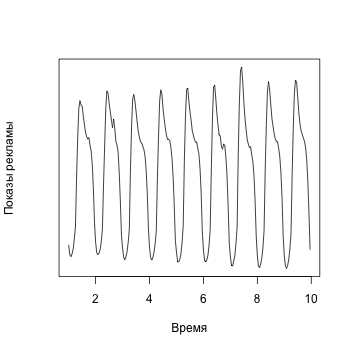
\includegraphics[scale=0.40]{images/examples_long_weekends}
\end{figure}
\end{frame}

\begin{frame}
\frametitle{Оценка параметров}

Длина ряда с предыдущего слайда 216 (то есть 9 суток). Применим к этому ряду метод SSA с окном 96. И оценим параметры периодичности по первым 10 компонентам (исключив тренд).

\begin{table}[h!]
\centering
 \begin{tabular}{||llc c|ll|}
 \hline
 Периоды & Фазы & Фазы (примерные) &  Амплитуды \\ [0.5ex]
 \hline\hline
 24 & 2.78 & $8\pi/9$ & 1.00  \\
 \hline
 12 & 1.55 & $\pi/2$ & 0.39  \\
 \hline
 8 & -1.56 & $-\pi/2$ & 0.13  \\
 \hline
 6 & -2.95 & $-15\pi/16$ & 0.11  \\
 \hline
\end{tabular}
\end{table}

Таким образом, модель периодической составляющей $s_i$ нашего ряда можно записать в следующем виде:
$$ s_i = \cos(\frac{2\pi}{24}i + \frac{8\pi}{9}) + 
                    0.39\cos(\frac{2\pi}{12}i + \frac{\pi}{2}) + 
                    0.13\cos(\frac{2\pi}{8}i - \frac{\pi}{2}) + 
                    0.11\cos(\frac{2\pi}{6}i - \frac{15\pi}{16}),$$
$\quad i = 1, \dots, n.$

\end{frame}


\begin{frame}
\frametitle{Оценка параметров}

В результате, модель сигнала (без шума) получилась внешне достаточно похожая на исходные реальные данные:

\begin{figure}
%\textbf{Сравнение реального и моделируемого рядов}\par\medskip
\includegraphics[scale=0.22]{images/real_vs_modelled}
\end{figure}
\end{frame}




\begin{frame}
\frametitle{Прочие параметры модели}

\begin{itemize}
	\item Длину ряда зафиксируем $n = 400$
	\item Значение тренда выберем нулевым: $c = 0$, то есть $t_i = 0, i = 1,\cdots, n$
	\item Параметры шума возьмем $\mu = 0, \sigma = 0.1$
\end{itemize}


\begin{itemize}
	\item Величины разладки $\delta^{(mean)*} \sim N(\mu = 0,\sigma = 0.2)$, $\delta^{(local)*} \sim N(\mu = 0,\sigma = 1)$;
	\item Минимальные допустимые значения разладок: $\delta^{(mean)*}_{min} = 0.3$, $\delta^{(local)*}_{min} = 0.5$;
	\item Место возникновения разладки зададим в середине ряда ряда $\tau = 216$
	\item Задержек выберем несколько $ d = (4, 24, 48)$
\end{itemize}

\begin{figure}
\textbf{Пример сгенерированного ряда с шумом и разладкой}\par\medskip
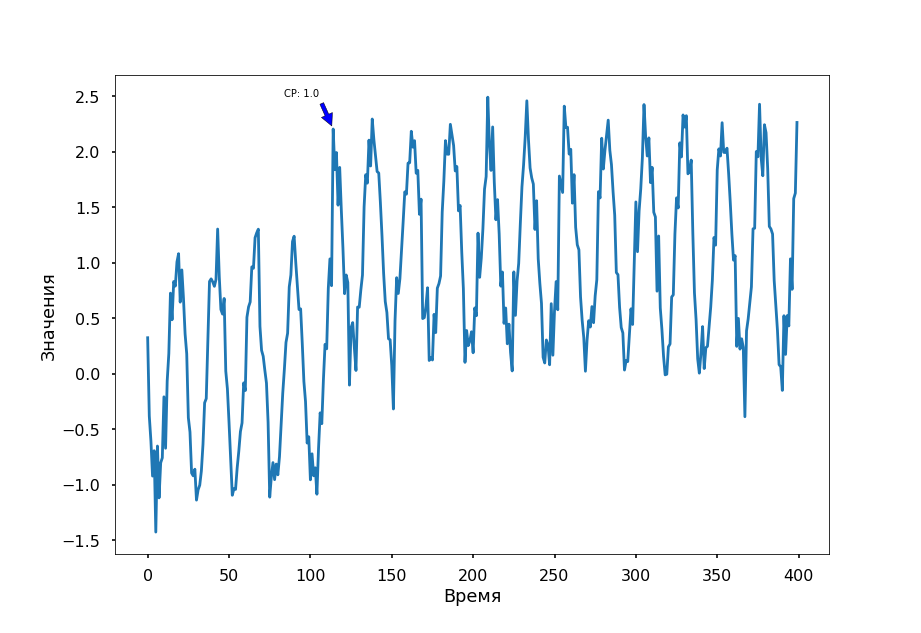
\includegraphics[scale=0.14]{images/data_modeling_example_2}
\end{figure}
\end{frame}


\section{Применение методов}

\begin{frame}
\frametitle{Моделирование рядов}

Попробуем применить, описанные выше модели к смоделированным данным.
\begin{itemize}
	\item Смоделируем 50 рядов
	\item У каждого ряда начало периодической компоненты выбирается случайно (то есть первый ряд может начинаться с нулевого часа, второй с пятого и т.п.). Это сделано, чтобы нивелировать влияние периодичности на оценку качества метода.
	\item Параметры методов выбраны следующие. Длина окна $l$ принимает значения 2, 4, 24, 48, 96. 
	\item Разладка возникает двух типов: локальная, разладка в среднем
%	\item Список значений порогов выбирается следующим образом. Моделируются 50 отдельных рядов (с разладкой и без) и на них запускается расчет значений функции разладки при заданном методе и заданных параметрах. Далее берется 95 квантиль из полученных значений. После чего берётся 100 значений в диапазоне от нуля до 95 квантили с равными промежутками.
\end{itemize}

\end{frame}

\begin{frame}
\frametitle{Методы}

И для подхода с аппроксимацией и для подхода с прогнозированием мы будем использовать следующие модели:

\begin{itemize}
	\item Среднее $f(x | b) = b $
	\item Четыре косинуса с периодами из модели генерации ряда  $f(x | P_i, p_i, \chi_i, b) = \sum_{i=1}^4P_i\cos(\frac{2\pi}{p_i}x + \chi_i) + b, $ где $p_1 = 24, p_2 = 12, p_3 = 8, p_4 = 6$
	\item Один косинус с периодом 24 + тренд $f(x | P, 24, \chi, b) = P\cos(\frac{2\pi}{24}x + \chi) + b $
	\item Среднее + тренд $f(x | b) = b + cx $
\end{itemize}

Таким образом, у нас есть 7 методов с одной стороны, и решетка параметров из 5 вариантов (длина окна $l$) с другой. Мы будем оценивать качество всех методов для комбинаций методов и параметров.

 \begin{alertblock}{Обратите внимание}
Методы, в которых лежит модель, отличная от среднего, бессмысленно применять для окон $l$ менее 48. Поскольку невозможно оценить какие либо параметры синуса, если длина ряда менее одного периода.
\end{alertblock}


%\begin{alertblock}{Обратите внимание}
%Следует отличать модель ряда, с помощью которого генерировался искусственный ряд и модель, используемая внутри метода обнаружения разладки.
%\end{alertblock}

\end{frame}

%\begin{frame}
%\frametitle{Методы}
%
%Всего будем сравнивать между собой 7 методов:
%\begin{itemize}
%	\item Аппроксимация с моделью из среднего
%	\item Аппроксимация с моделью из четырёх синусов с периодичностью 24, 12, 8, 6
%	\item Аппроксимация с моделью из одного синуса с периодичностью 24
%	\item Аппроксимация с моделью только из среднего и тренда (для проверки, что добавление лишнего в модель ломает метод)
%	\item Прогнозирование с моделью из среднего
%	\item Прогнозирование с моделью из четырёх синусов с периодичностью 24, 12, 8, 6 
%	\item Прогнозирование с моделью из одного синуса с периодичностью 24
%%	\item Базовая простая модель, в которой функция разладки это прирост текущих значений к значениям аналогичных часов сутки назад.
%\end{itemize}
%
%\end{frame}


%\begin{frame}
%\frametitle{Замечания}
%
%Поскольку у нас есть 7 методов с одной стороны, и решетка параметров из 5 вариантов (длина окна $l$) с другой, то мы будем оценивать качество всех методов для комбинаций методов и параметров.
%
%Однако не во всех случаях корректно применять методы, поэтому проговорим исключения, когда мы не будем считать качество:
%\begin{itemize}
%	\item Методы, в которых лежит модель, отличная от среднего, бессмысленно применять для окон $l$ менее 48. Поскольку невозможно оценить какие либо параметры синуса, если длина ряда менее одного периода. 
%	\item В случае с разладкой в тренде бессмысленно применять методы  с окном $l$ менее 48 по тем же причинам
%\end{itemize}
%
%\end{frame}


\begin{frame}
\frametitle{Результаты}

В таблице приведены сводные результаты ROC-AUC для экспериментов на 50 временных рядах.

\begin{figure}
\textbf{Результаты применения методов к смоделированным данным}\par\medskip
\includegraphics[scale=0.30]{images/results_pivot}
\end{figure}


\end{frame}


\begin{frame}
\frametitle{Выводы}

%\begin{itemize}
%	\item Как мы видим, лучше всего сработал метод аппроксимации с моделью „Среднее“. Причем для разных типов разладки. Однако для каждого типа разладки у этого метода своя оптимальная длина окна
%	\item Также, хорошо сработал метод аппроксимации с моделью из четырех синусов
%	\item Методы прогнозирования с моделями „Среднее“ и „4 синуса + тренд“ сработали хорошо, но немного хуже чем методы аппроксимации
%	\item Базовый простой метод (в таблице это "naive") показал себя плохо. Причина тут в том, что наш ряд колеблется около нуля. Соответственно любые отклонения от нуля могут иметь очень большой прирост за счет эффекта низкой базы. Из-за этого базовый метод вероятно сработал бы неплохо в случае ряда с ненулевым средним, но в нашем случае он сработал плохо.
%	\item Примечательно, что все методы хорошо определяют разладку в тренде, если выбрать окно $l=96$. Вероятно имеет смысл понизить величину разладки при генерации ряда.
%	\item Плохо сработали методы с моделью „Синус + тренд“ и с моделью „Тренд“(и аппроксимация и прогнозирование).

%\end{itemize}

\end{frame}

\end{document}
